\section{How to visualise the result of the change detection algorithm? (\ref{rq:how-to-visualise-result} )} \label{rq:type-visualisation-answer}

In section \ref{sec:finding-changes} the detection of changes between two versions of the same application is explained. It showed that abstract states were used to find corresponding states between two models. The corresponding states were compared to discover the changes in element data. In this section, the change detection results are used as input for visualising the changes. 

In this section, the visualisation of the change detection results is discussed. First, the technology is discussed how to show a graph and what is needed for that (section \ref{sec:graph-visualisation}). Section \ref{sec:merge-graph} explains how the results are used to merge the two graphs and to visualise one single \textit{merge graph}.

\subsection{How are graphs visualised} \label{sec:graph-visualisation}

The visualisation of graphs in the new analysis tool is being drawn by Cytoscape.js\footnote{https://js.cytoscape.org/}. "Cytoscape.js is an open-source graph theory (a.k.a. network) library written in JS [JavaScript]" \cite{cytoscape-js}. The cytoscape.js library was used by the build-in analysis website of \testar, created by Mulder \cite{thesisMulders} and was migrated to the new Analysis website. The Java code used to convert the data from OrientDb to a Cytoscape.js acceptable format has been refactored and moved to the new C\# code.

All the information about a model and graph is stored in OrientDB. The new Analysis website retrieves the model and graph data through the \testar .NET server from the OrientDB database. This communication is done by the \verb|GraphEngine|. The \verb|GraphEngine| contains a method for each \testar layer, for example: \verb|FetchAbstractLayerAsync|. Edges between layers are retrieved with a different method, like, \verb|FetchAbstractConcreteConnectors|, which retrieves the edges between an abstract and concrete state. Splitting up the methods for each layer makes it possible to retrieve each layer individually. For example, the graph shown for an application, like in figure \ref{fig:graph-page}, needs all the information, while the detection algorithm only needs the abstract information. 

The \verb|GraphEngine| retrieves the data from each layer and transforms them into an internal model. A UML class diagram of the internal model can be viewed in figure \ref{fig:class-diagram-models} (the \verb|AppGraph| does not play a role in displaying the graph). When the transformation from the OrientDB database to graph elements is completed, the engine returns them in a list structure. 

Beside the vertexes and edges, the \verb|GraphEngine| can also include a compound object. A compound object group graphs objects together. Figure \ref{fig:compound-example} shows a compound layer that groups the concrete states into the group 'ConcreteLayer'. The new Analysis website has options on the settings page to enable the grouping of items into a compound layer or not.

\begingroup
\captionsetup{type=figure}
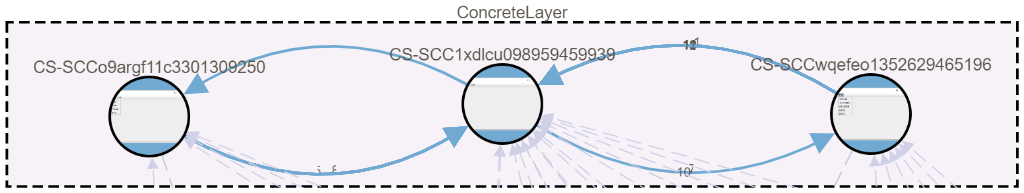
\includegraphics[scale=0.6]{content/5-Results/Images/compound-layer.png}
\captionof{figure}{Compound object grouping concrete states together}\label{fig:compound-example}
\endgroup

After the list with \verb|GraphElement|'s is retrieved, it must be passed to the Cytoscape.js library in JSON objects. Since the \verb|GraphElement| is created with the idea of JSON in mind, the serialisation to JSON is easy. An example of the serialisation result can be viewed in listing \ref{code:graph-json}. The data contains an array of elements each having three attributes: \verb|group|, \verb|data| and \verb|classes|. The \textit{group} either contains the value nodes or edges, representing their graph element. The attribute \verb|data| contains the \verb|id| of the element and all the additional data about the vertex/edge. For an edge, that data also contains the target and source id, specifying the id of two specific vertices. The element classes are similar to classes in \textsc{CSS} and can be used to style the elements in the GUI. 

The result of listing \ref{code:graph-json} generates the graph visible in figure \ref{fig:graph-example}. The full HTML code is added as appendix \ref{appendix:cytoscape-example}. 

\begingroup
\captionsetup{type=figure}
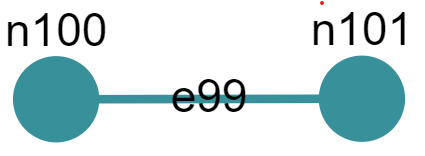
\includegraphics[scale=0.6]{content/5-Results/Images/graph-example.png}
\captionof{figure}{Example graph}\label{fig:graph-example}
\endgroup

\newpage
\begin{lstlisting}[language=xml, caption=Graph representation in JSON, label=code:graph-json]
[
  {
    "group": "nodes",
    "data": {
      "id": "n100" 
    },
    "classes":[
      "AbstractState"
    ]
  },
  {
    "group": "nodes",
    "data": {
      "id": "n101"
    },
    "classes":[
      "AbstractState"
    ]
  },
  {
    "group": "edges",
    "data": {
      "id":"e99",
      "target": "n100",
      "source": "n101"
    },
    "classes" :[
      "AbstractAction"
    ]
  }
]
\end{lstlisting}

\subsection{Merging the two graphs} \label{sec:merge-graph}

After the two models are compared by the change detection algorithm (section \ref{sec:change-detection-algorithm}), a graph containing both models and the changed detection results can be created. The technique presented by Andrews et al. \cite{andrews2009visual} is used to merge two graphs into one merge graph. Andrews et al. describe a six steps approach to merging two graphs. The algorithm for merging will be explained below in the same six steps.

\subsubsection{1. Read Two input Graphs}

The two models and the two graphs need to be read. Section \ref{sec:graph-visualisation} explains how the graphs $G_{old}$ and $G_{new}$ are read.

\subsubsection{2. Find Matching Nodes}
This step is handled by the change detection algorithm discussed in section \ref{sec:change-detection-algorithm}.
Results are an enriched version of $G_{old}$ and $G_{new}$. 


\subsubsection{3. Create Merge Graph}
Andrews et al. use the following algorithm to merge two graphs into a merge graph: "A merge graph $G_m$ is created by combining the two input graphs [$G_{old}$ and $G_{new}$] and considering the matches from $S_m$ [In our case $S_m$ does not exist. Instead the corresponding ids between states is used to match nodes in the graph]. First all nodes and edges from $G_{new}$ are added to $G_m$. Then all non-matching nodes from $G_{old}$ are added to $G_m$. Finally all edges from $G_{old}$ are added to $G_m$ and wired, except the edges with the same actionId. Edges which connect to matching nodes from $G_{old}$ have to be connected to the matching nodes from $G_{new}$." \cite{andrews2009visual}. \footnote{Andrews et al. used $G_1$ and $G_2$ to indicate their graphs, the names have been replaced with $G_{old}$ and $G_{new}$}

The edges leading to nodes in $G_{old}$ need to be rewired to nodes in $G_{new}$. Two in-memory dictionaries are used for the rewiring process. The first dictionary contains the combination of $StateId_{old}$ with $NodeId_{new}$. The second dictionary contains the combinations of $NodeId_{old}$ with $StateId_{old}$. A combination of the following can be made using the two dictionaries:
\[ NodeId_{old} \rightarrow  StateId_{old} \rightarrow NodeId_{new}. \]
Since the edges contain the Id of both the target and source node, using the two dictionaries, the $NodeId_{old}$ can be rewired to $NodeId_{new}$.

\subsubsection{4. Lay Out Merged Graph}

Laying out the merged graph is handled by the Cytoscape.js library as discussed in section \ref{sec:graph-visualisation}.

\subsubsection{5. Propagate Changes to Original Graphs}

The original graphs are not displayed in the comparison results. Doing so would take up too much screen space, especially when the graphs can become very big. New classes are added to the graph elements in the merge graph to provide the option to view the original graphs.

First of all, the nodes from $G_{new}$ are given the class 'NewVersion', and if they had a corresponding state, the class 'OldVersion', since the matching nodes from $G_{old}$ are not added to the $G_m$. The same is done for all the edges in $G_{new}$. The non-matching nodes and all the edges in $G_{old}$ are given the class 'OldVersion'.

The 'NewVersion' and 'OldVersion' filtering can be applied by Cytoscape.js, making it possible to toggle the view into the Old, New and Merge views. 

\subsubsection{6. Manually Edit merged graph}

This section does not apply to the New Analysis Website since it does not provide an option to set corresponding states to change the merged graph manually. 